%!TEX root = ../thesis.tex
\chapter{Appendix}
\label{app:appendix}




-> Partitioning of SAFT: Data -> How to put Data on GPU -> What limitations -> Hardware -> COmputation Time

Paper: Find paper which shows requrements on tissue resolution-> What resolution of our vectors in each direction neccessary? -> WHat requirements on the HW then?
How much Data will come out?
WHy not feasable? WHat do differently?

-> Review of partitioning problem on GPU  -> In z-slices
Implementation small in MATLAB for verification
->
-> WHat Limits came up?
-> How to circumvent those limitations?








\section{Alternative identification of faces}
For the analysis of the direction-dependent reflection characteristics each \ac{ascan} has to be assigned to a certain direction of the voxel.
Depending on which geometry was chosen for the segmentation of the volume there is a set of normals which are orthogonal to each face of the geometry. To assign a face to each \ac{ascan} it makes sense to calculate the angle $\angle (\overrightarrow{a},\overrightarrow{b})$ between the direction vector and each normal.


\begin{equation}
\centering
\angle (\overrightarrow{a},\overrightarrow{b}) = \varphi
\label{eqation_angle}
\end{equation}


\begin{equation}
\centering
cos(\varphi )  =   \frac{(\overrightarrow{a} \cdot \overrightarrow{b})}{\left \| \overrightarrow{a} \right \|_2  \cdot \left \| \overrightarrow{b} \right \|_2}
\label{eqation_cos_phi}
\end{equation}

\begin{equation}
\angle (\overrightarrow{a},\overrightarrow{b}) = 
cos^{-1} \left (  
\frac{(\overrightarrow{a} \cdot \overrightarrow{b})}{\left \| \overrightarrow{a} \right \|_2  \cdot \left \| \overrightarrow{b} \right \|_2} 
\right )
\label{eqation_angle_final}
\end{equation}

To identify the face which belongs to the corresponding \ac{ascan} the smallest angle of the set has to be found.

\qquad





For every emitter-receiver combination, for each voxel and each rotation position of the aperture one calculation of the angle between two vectors has to be performed. Depending on which geometry is used for every normal of the faces of the geometry this calculation hast to be repeated. The number of calculations results in:

\boxed{ \# Calculations = \#Voxel \cdot \#Emitter \cdot \#Receiver \cdot \#AperturRotation \cdot \#Faces}

For the case of using a 12 face dodecahedron, 628 emitters, 1413 receivers, only a single slice of 1024x64 voxels and ten aperture positions already $[628 \cdot 1413 \cdot 1024 \cdot 64 \cdot 10 \cdot 12] = 6.98x10^{12}$ calculations have to be  performed to find the smallest angle index. By decreasing the complexity of these calculations the performance of the reconstruction algorithm can be greatly improved. To reduce the computational cost it is not necessary to calculate the absolute angle between each vector combination. It simply can be proven that for certain circumstances one certain combination of direction vector and face-normal has the smallest angle of the available set. The following segment is adapted from \cite{PatrickHucker2014EvaluationRuckstreumodells} and some inaccuracies were corrected.

\qquad

In the following $\overrightarrow{v}$ is the direction vector from the \ac{ascan} which should be matched best to one of the norm vectors $\overrightarrow{n_i}$ from the $N$ faces of the used geometry.


\begin{equation}
\angle (\overrightarrow{v},\overrightarrow{n_i}) =  cos^{-1}\left (    \frac{(\overrightarrow{v} \cdot \overrightarrow{n_i})}{\left \| \overrightarrow{v} \right \|_2  \cdot {\left \| \overrightarrow{n_i} \right \|_2}}  \right ) 
\label{equation_with_v_n}
\end{equation}



For the first simplification we can neglect the $arccos$ in equation \ref{equation_with_v_n}. Since the arccosine is monotonically decreasing in the interval $[-1,1]$ (Figure \ref{accos_figure}) only the argument of the $arccos$ has to be regarded to find the smallest angle $\angle (\overrightarrow{v},\overrightarrow{n_i})$. To reach a small value for the arccosine function its argument has to become as big as possible.
\begin{equation}
min \left (  \angle (\overrightarrow{v},\overrightarrow{n_i}) \right ) =  max \left (    \frac{(\overrightarrow{v} \cdot \overrightarrow{n_i})}{\left \| \overrightarrow{v} \right \|_2  \cdot {\left \| \overrightarrow{n_i} \right \|_2}}  \right ) 
\label{equation_acos_neglect}
\end{equation}

\begin{figure}[H]
    \centering
    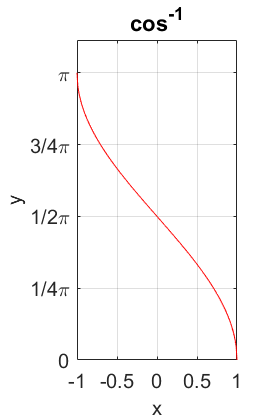
\includegraphics[width=0.3\textwidth]{accos.png}
    \caption{ Monotonically decreasing arccosine function.}
    \label{accos_figure}
\end{figure}

Since the euclidean norm of a normal vector $\left \| \overrightarrow{n_i} \right \|_2 = 1 , \forall i \in [1,...,N]$, the equation \ref{equation_acos_neglect} can be simplified further:


\begin{equation}
min \left (  \angle (\overrightarrow{v},\overrightarrow{n_i}) \right ) =  max \left (    \frac{(\overrightarrow{v} \cdot \overrightarrow{n_i})}{\left \| \overrightarrow{v} \right \|_2  \cdot { \underset{=1}{\underbrace{\left \| \overrightarrow{n_i} \right \|_2}}} }  \right ) = 
max \left (    \frac{(\overrightarrow{v} \cdot \overrightarrow{n_i})}{\left \| \overrightarrow{v} \right \|_2  }  \right )
\label{equation_acos_norm_simply}
\end{equation}

During the search of the smallest angle between the direction vector $\overrightarrow{v}$ and the set of normal vectors $\overrightarrow{n_i}$ the direction vector $\overrightarrow{v}$ does not change. 
The norm of the direction vector $\left \| \overrightarrow{v} \right \|_2$ is the same in every iteration of the search, thus has no influence on the final result and therefore can be remove from the formula.

\begin{equation}
min \left (  \angle (\overrightarrow{v},\overrightarrow{n_i}) \right ) = 
max \left (    \frac{(\overrightarrow{v} \cdot \overrightarrow{n_i})}{\left \| \overrightarrow{v} \right \|_2  }  \right ) = max \left (    \overrightarrow{v} \cdot \overrightarrow{n_i}  \right ) 
\label{equation_other_norm_simply}
\end{equation}

The final problem arises from equation \ref{equation_other_norm_simply}. The goal is to find the index $i_0$ for which the product of the direction vector $\overrightarrow{v}$ and the normal $\overrightarrow{n_{i_0}}$ is maximised: 

\begin{equation}
i_0 = \underset{i \in 0..N}{\mathrm{argmax}} \left (    \overrightarrow{v} \cdot \overrightarrow{n_i}  \right )
\label{equation_arg_max}
\end{equation}




\section{Spherical coordinate system}
Spherical coordinates are used to create test vectors for evaluating the algorithms. Depending on the available computation power and memory it is possible to create as many normals as possible to cover as many possible directions as possible.

\bigskip
In three dimensions the spherical coordinate system consists of a radius $r$, and inclination $\vartheta$ and an azimuth $\varphi$. The conversion from one coordinate systems to the other can be seen in tables \ref{table_pol_to_cart} and \ref{table_cart_to_Pol}.

\begin{figure}[H]
  \centering
  \begin{minipage}[b]{0.45\textwidth}
    \centering
  \fbox{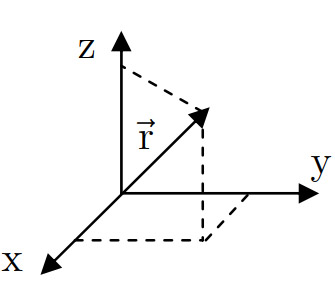
\includegraphics[width=0.75\linewidth]{cartesian_coord.jpg}}
  \caption{Cartesian coordinate system \cite{Prof.Dr.-Ing.GertF.Trommer2013FelderWellen}.}
  \end{minipage}
  \hfill
  \begin{minipage}[b]{0.45\textwidth}
    \centering
  \fbox{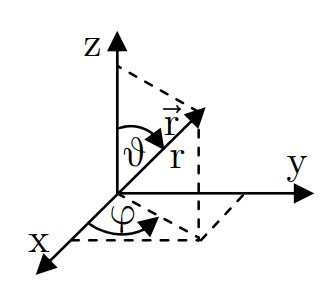
\includegraphics[width=0.75\textwidth]{polar_coord.jpg}}
  \caption{Spherical coordinate system \cite{Prof.Dr.-Ing.GertF.Trommer2013FelderWellen}.}
  \end{minipage}
    \hfill
\label{polar_cart_systems}
\end{figure}




\begin{table}[H]
\centering
\begin{tabular}{|ll|}
\hline
\textbf{Cartesian coordinate system} & \textbf{Spherical coordinate system}                                                                            \\ \hline
$x $                            & $= r \cdot sin(\vartheta) \cdot cos(\varphi)$ \\
$y $                            & $= r \cdot sin(\vartheta) \cdot sin(\varphi)$ \\
$z $                            & $= r \cdot cos(\vartheta)$                                                  \\ \hline
\end{tabular}
\caption{Conversion of polar coordinates to Cartesian coordinates  \cite{Bronstein2005TaschenbuchMathematik}.}
\label{table_pol_to_cart}
\end{table}


\begin{table}[H]
\centering
\begin{tabular}{|ll|}
\hline
\textbf{Cartesian coordinate system} & \textbf{Spherical coordinate system}                                                                            \\ \hline
$\sqrt{x^2+y^2+z^2} $                               & $= r$ \\
$arctan( \frac{\sqrt{x^2+y^2}}{z} ) $  & $= \vartheta$ \\ 
$arctan( \frac{y}{x} ) $               & $= \varphi$                                                  \\ \hline
\end{tabular}
\caption{Conversion of Cartesian coordinates to polar coordinates \cite{Bronstein2005TaschenbuchMathematik}. }
\label{table_cart_to_Pol}
\end{table}




%\section{Performance improvement by GPU}

%In the paper \cite{Gohringer2011ReconfigurableEvaluation} the reconstruction was performed on a CPU, a \ac{gpu} as well as an FPGA. One step of the reconstruction took $150\mu \sec$ for the CPU. The \ac{gpu} managed the same calculation in $3,23 \mu \sec$ whereas the FPGA needed $144 \mu \sec$ to complete the calculation. Therefore, the paper concludes that the \ac{gpu} achieves the highest performance when it comes to the reconstruction of \ac{usct}-images. 


%\section{Treatment of breast cancer}

%One form of possible treatment of breast cancer is the mastectomy. During this procedure big parts of the breast tissue as well as parts of the lymphatic system near the armpit are surgically removed (figure \ref{mastecto_example_picture}).  


%\begin{figure}[H]
   % \centering
%    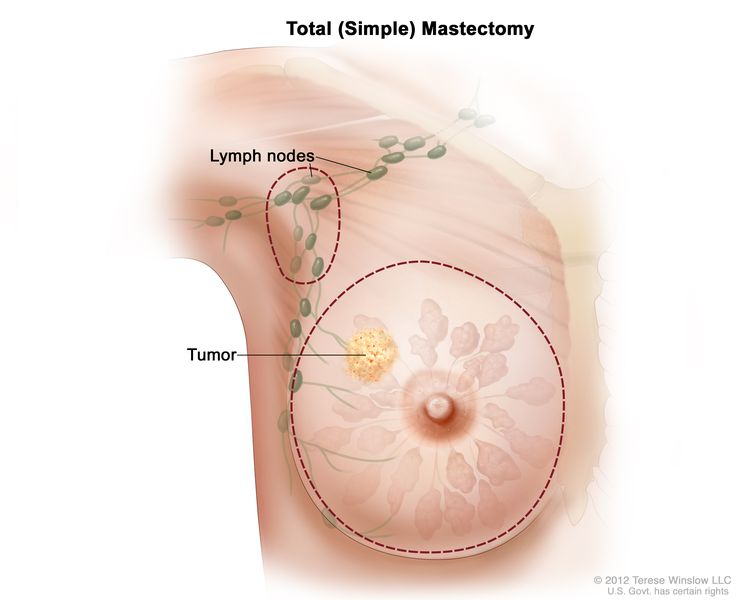
\includegraphics[width=0.75\textwidth]{Graphics/Mastectomy.jpg}
%    \caption{Treatment of female breast cancer. During the mastectomy big parts of the breast are surgically removed (marked by dotted line). Picture source: \cite{NationalInstitutesofHealthNIH-NationalCancerInstituteNCIBreastTreatment}. }
 %   \label{mastecto_example_picture}
%\end{figure}

%This treatment may be combined with chemo therapy to decrease the size the tumour prior to the surgery. The post operative therapy often consists of radiation and hormone therapy to remove any cancer cells that might be left after the the mastectomy \cite{NationalInstitutesofHealthNIH-NationalCancerInstituteNCIBreastTreatment}.
%This further motivates the use of early screening technologies to detect possible tumours before a chemo therapeutic treatment is necessary.




%\section{Imaging techniques}
%\label{Imaging_techniqe}


%For the regular mammographic screenings typically X-ray-based imaging techniques are in use. The breast has to be compressed between two plates so that a higher contrast of the breast tissue can be archived (see Figure \ref{mammo_example_picture}). Besides the advantages of delivering results shortly after the screening and by having a high enough resolution to detect small tumour cells before they are detectable by palpation, there are certain downsides that have to be considered.
%The biggest problem with X-ray-based mammographic screenings is the usage of ionising radiation. When it comes to x-ray and gamma radiation there is no such thing as a safe dose. Every dose of ionizing radiation of for example a low-dose X-ray mammography has proven to add to the incidence of breast cancer  \cite{Pauwels2015BreastRadiobiology} and so the main objective is the reduction of exposure to ionizing radiation.

%\begin{figure}[H]
 %   \centering
  %  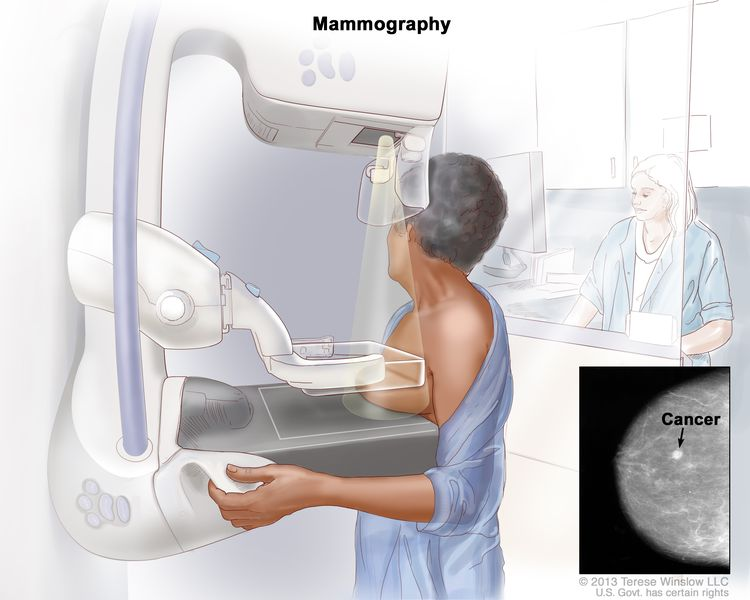
\includegraphics[width=0.75\textwidth]{mammography.jpg}
 %   \caption{Schematic of the mammography procedure. The breast is pressed between two plates and a beam of X-Ray-Radiation is used to produce the picture. On the bottom right is an example image of a female breast with the white dot indicating cancerogenous tissue. Picture source: \cite{NationalInstitutesofHealthNIH-NationalCancerInstituteNCIBreastTreatment}. }
 %   \label{mammo_example_picture}
%\end{figure}

%Another screening method which is not an imaging technique is the physical examination of the breast either by the patient herself or during a clinical breast exam performed by a health professional. For this method the breast is carefully palpated to check for lumps or any kind of anomaly that might indicate an early stage of breast cancer. This method has one major disadvantage: lumps can only be detected by palpation after they have reached a certain size which, compared to the size of detectability during a mammography screening, is relatively large. Thus, the potential diagnosis of breast cancer solely by palpation often leads to the identification of first cancer symptoms in a later stage compared to mammography or \ac{usct} screening.

%\bigskip

